\chapter{Application}
\label{chap:ch4}

\section{Analysis}

\subsection{Functional requirements}

\par Throughout the application, the user can do the following:

\begin{itemize}
    \item Unauthenticated user
    \begin{itemize}
        \item Create an account
        \item Login into the application
        \item Reset their account's password
    \end{itemize}
    \item Regular user
    \begin{itemize}
        \item Log out of the application
        \item Change between light and dark theme
        \item Visualize, search, sort and filter attractions
        \item Add a new attraction or edit a created one
        \item React to an attraction with like or dislike
        \item Save an attraction to a new or existing collection
        \item Share an attraction to Threads, Twitter, Email or copy its link
        \item View an attraction's details on its page
        \item Comment on an attraction's page
        \item View their own and other users' profile
        \item Add or change their profile photo and description
        \item Send, accept and decline friend requests and unfriend current friends
        \item View their own and other users' friends
        \item View their own sent or received friend request
        \item View the list of their created attractions
        \item View the list of their collections
        \item Reorder their list of collections
        \item Add a new collection or edit/delete a created one
        \item View the details of a collection
        \item Reorder attractions within a collection
        \item Delete an attraction from the collection
        \item Set the picture of an attraction as the collection's picture.
    \end{itemize}
    \item Admin
    \begin{itemize}
        \item Anything a regular user can do
        \item View the list of attraction types and how many attractions are using them
        \item Add or rename attraction types
        \item Delete unused attraction types
    \end{itemize}
\end{itemize}


\subsection{Use cases}

\begin{figure}[!ht]
    \centering
    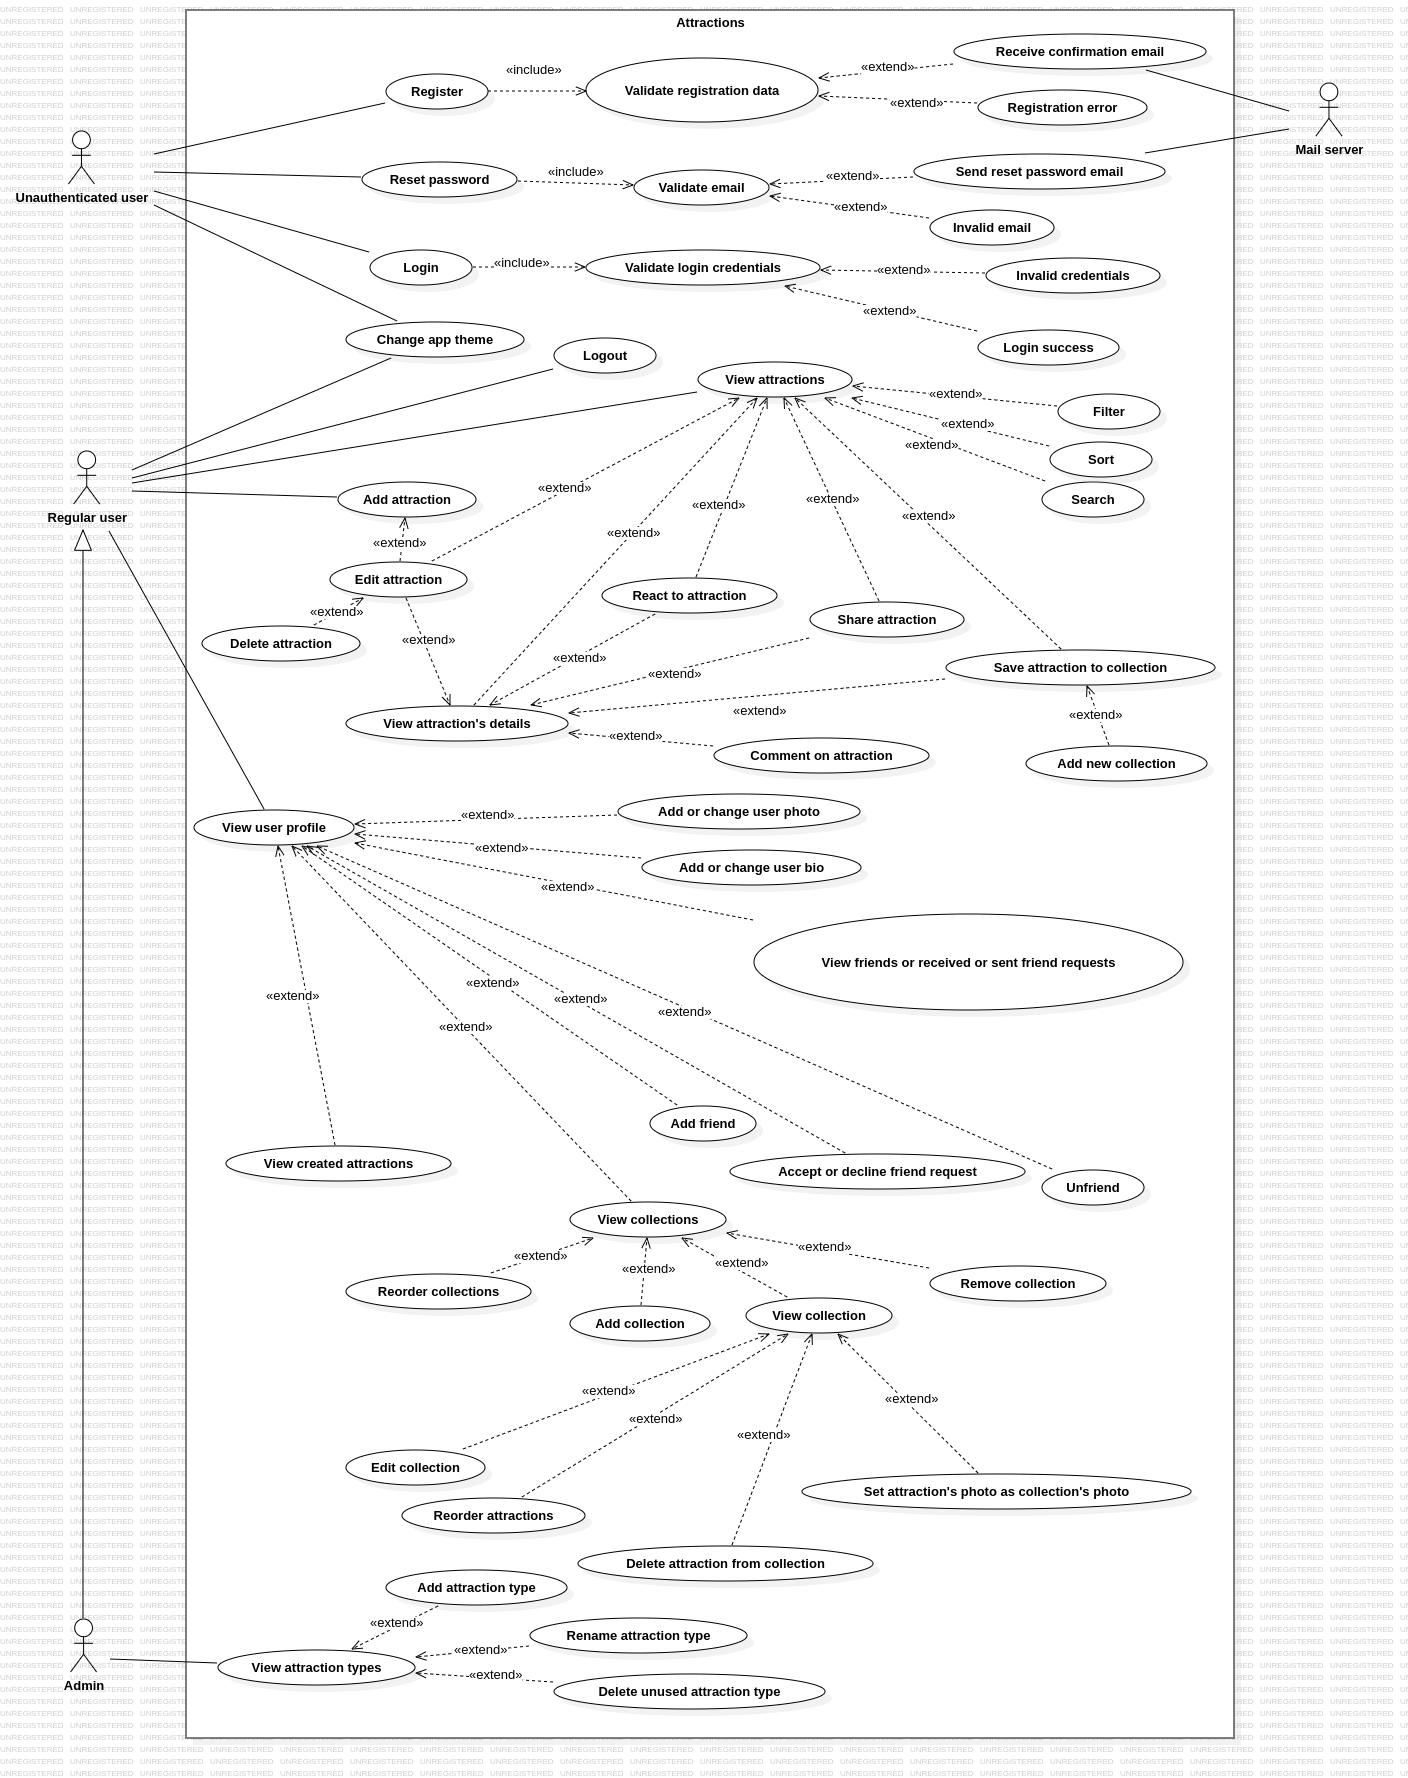
\includegraphics[width=1\linewidth]{UseCaseDiagram1.png}
    \caption{Use case diagram}
    \label{fig:enter-label}
\end{figure}

\clearpage % https://www.overleaf.com/learn/latex/Questions/How_can_I_get_my_table_or_figure_to_stay_where_they_are%2C_instead_of_going_to_the_next_page%3F

\begin{table}[!ht]
    \centering
    \begin{tabular}{|l|p{11cm}|}
        \hline
        \multicolumn{2}{|c|}{Use case: Register} \\
        \hline
         Actors & Regular User \\
        \hline
        Standard process & 
            % {\rowcolors{3}{green!20!yellow!50}{green!10!yellow!40}
            {\rowcolors{3}{gray!40}{gray!20}
                \begin{tabular}{|c|p{4.5cm}|p{4.5cm}|}
                    \multicolumn{3}{c}{} \\
                    \hline
                    No. & User action & System response \\
                    \hline
                    1 & User enters username, email and password then clicks the "Register" button & \\
                    \hline
                    2 &  & The systems validates the data, creates the account, sends the confirmation email and then displays a notification \\
                    \hline
                \end{tabular}
            } 
            \begin{tabular}{|c|p{4.5cm}|p{4.5cm}|}
                \multicolumn{3}{c}{} \\
            \end{tabular}
            \\
        \hline
         Alternative process & 
            {\rowcolors{3}{gray!40}{gray!20}
                \begin{tabular}{|c|p{4.5cm}|p{4.5cm}|}
                    \multicolumn{3}{c}{  } \\
                    \hline
                    No. & User action & System response \\
                    \hline
                    1 & User enters username, email and password then clicks the "Register" button & \\
                    \hline
                    2 &  & The systems validates the data, finds validation problems and shows the user the problems with each registration fieldd \\
                    \hline
                \end{tabular}
            } 
            \begin{tabular}{|c|p{4.5cm}|p{4.5cm}|}
                \multicolumn{3}{c}{} \\
            \end{tabular}
            \\
        \hline
         Preconditions & The user must be on the register page \\
        \hline
         Postconditons & If the registration is successful, the user will receive a confirmation email \\
        \hline
    \end{tabular}
\end{table}

\section{Architecture}

\par The application is structured on the client - server model. The client is a web application created using React and the server is a Web API created using the ASP.NET Core subset of the .NET Framework. For persistent storage the database used is SQLite. External services are used for email sending and photo upload.

\begin{figure}[!ht]
    \centering
    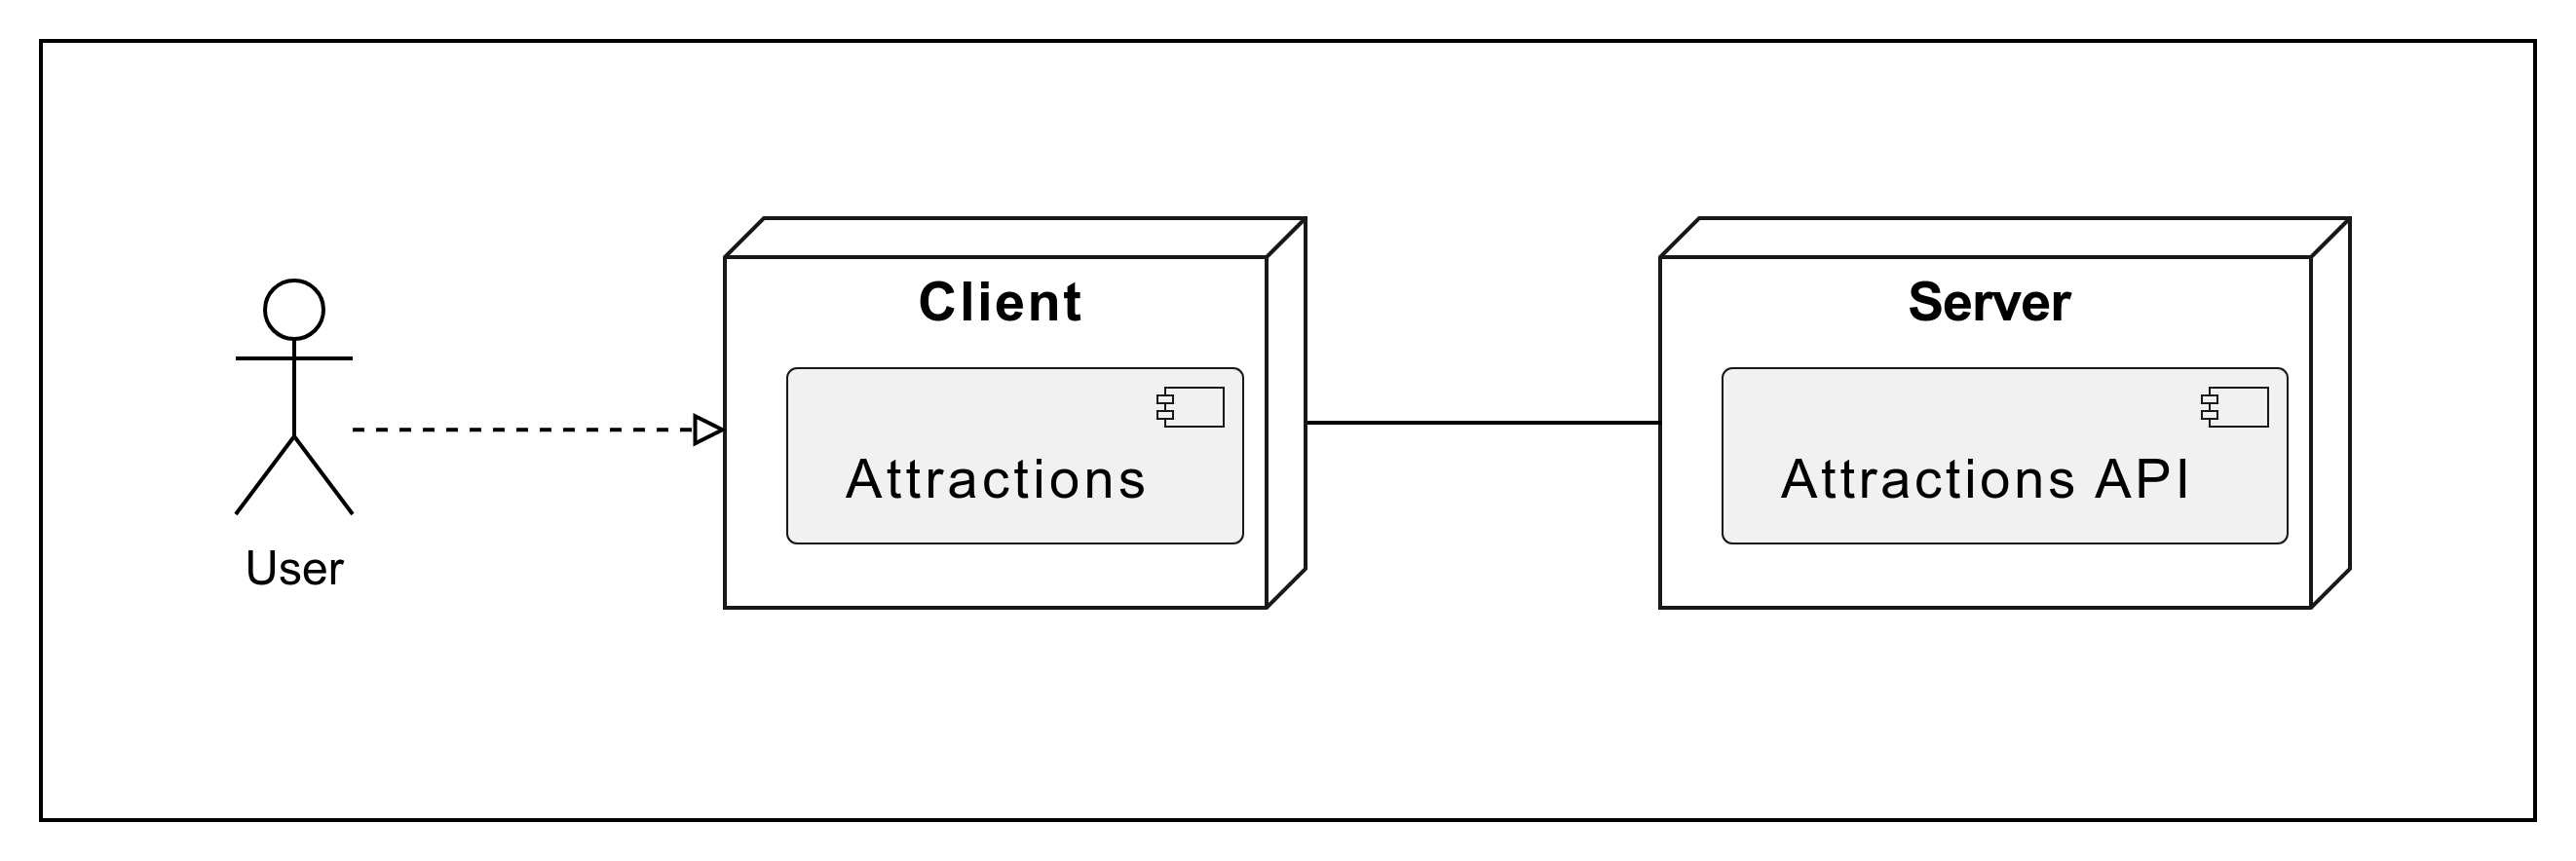
\includegraphics[width=1\linewidth]{app-architecture.png}
    \caption{Application architecture}
    \label{fig:enter-label}
\end{figure}

\begin{figure}[!ht]
    \centering
    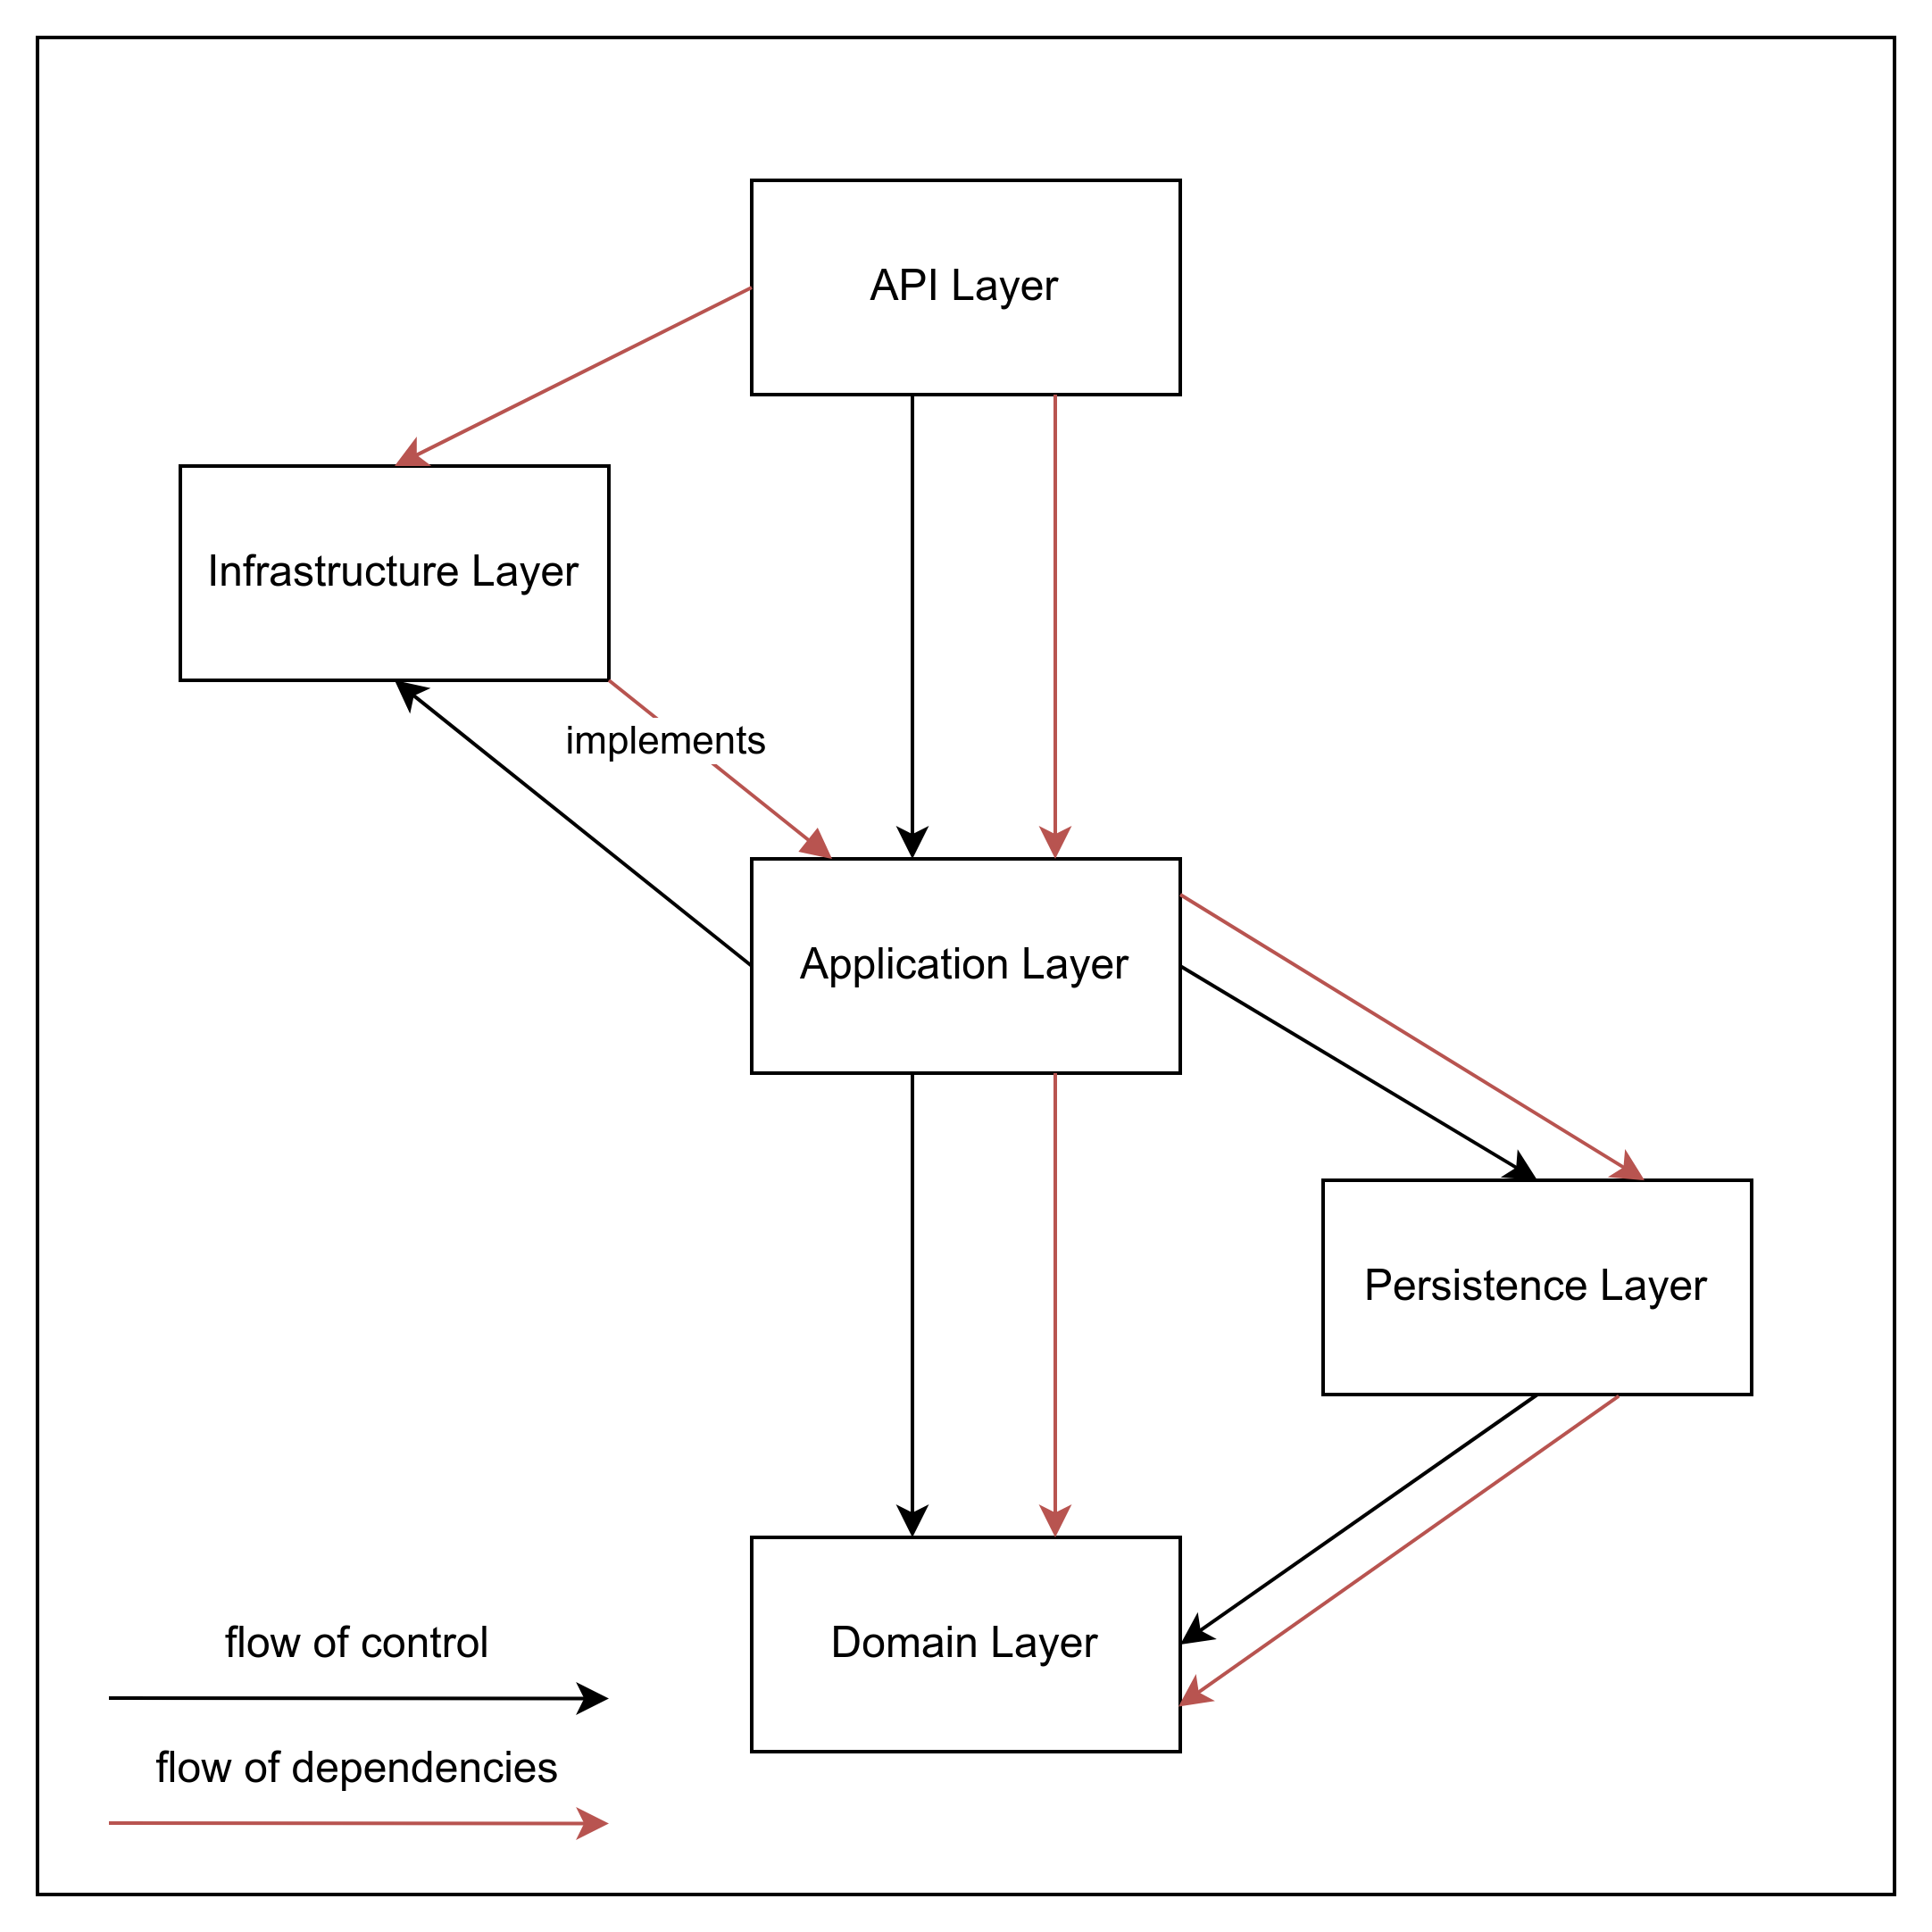
\includegraphics[width=0.96\linewidth]{backend-layers-with-flow-of-control.png}
    \caption{Backend layers}
    \label{fig:enter-label}
\end{figure}


\subsection{Diagrams}

\subsubsection{Domain class diagram}

\begin{figure}[!ht]
    \centering
    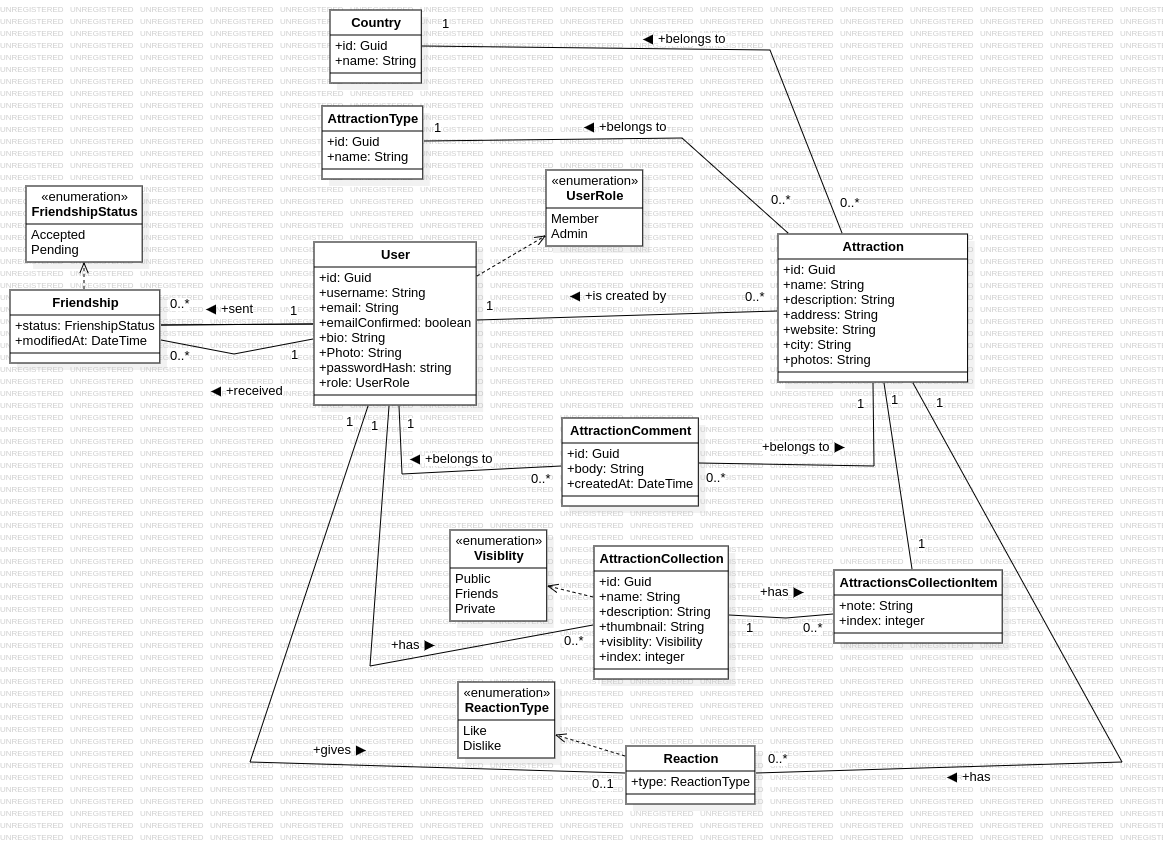
\includegraphics[width=1\linewidth]{domain-class-diagram.png}
    \caption{Domain class diagram (*associations should be aggregations)}
    \label{fig:enter-label}
\end{figure}

\subsubsection{Database diagram}

\par Since the database is generated by the Entity Framework, its structure is similar to the domain:

\clearpage % https://www.overleaf.com/learn/latex/Questions/How_can_I_get_my_table_or_figure_to_stay_where_they_are%2C_instead_of_going_to_the_next_page%3F

\begin{figure}[!ht]
    \centering
    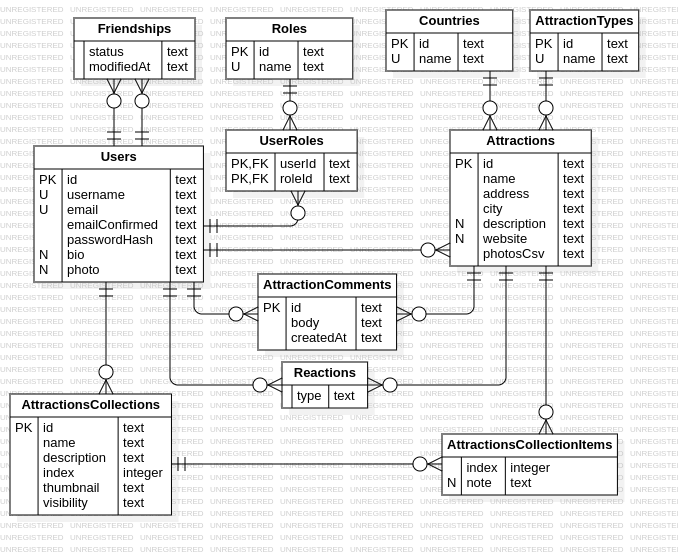
\includegraphics[width=0.7\linewidth]{db-diagram.png}
    \caption{Database diagram}
    \label{fig:enter-label}
\end{figure}


\subsubsection{Business logic class diagram}

\begin{figure}[!ht]
    \centering
    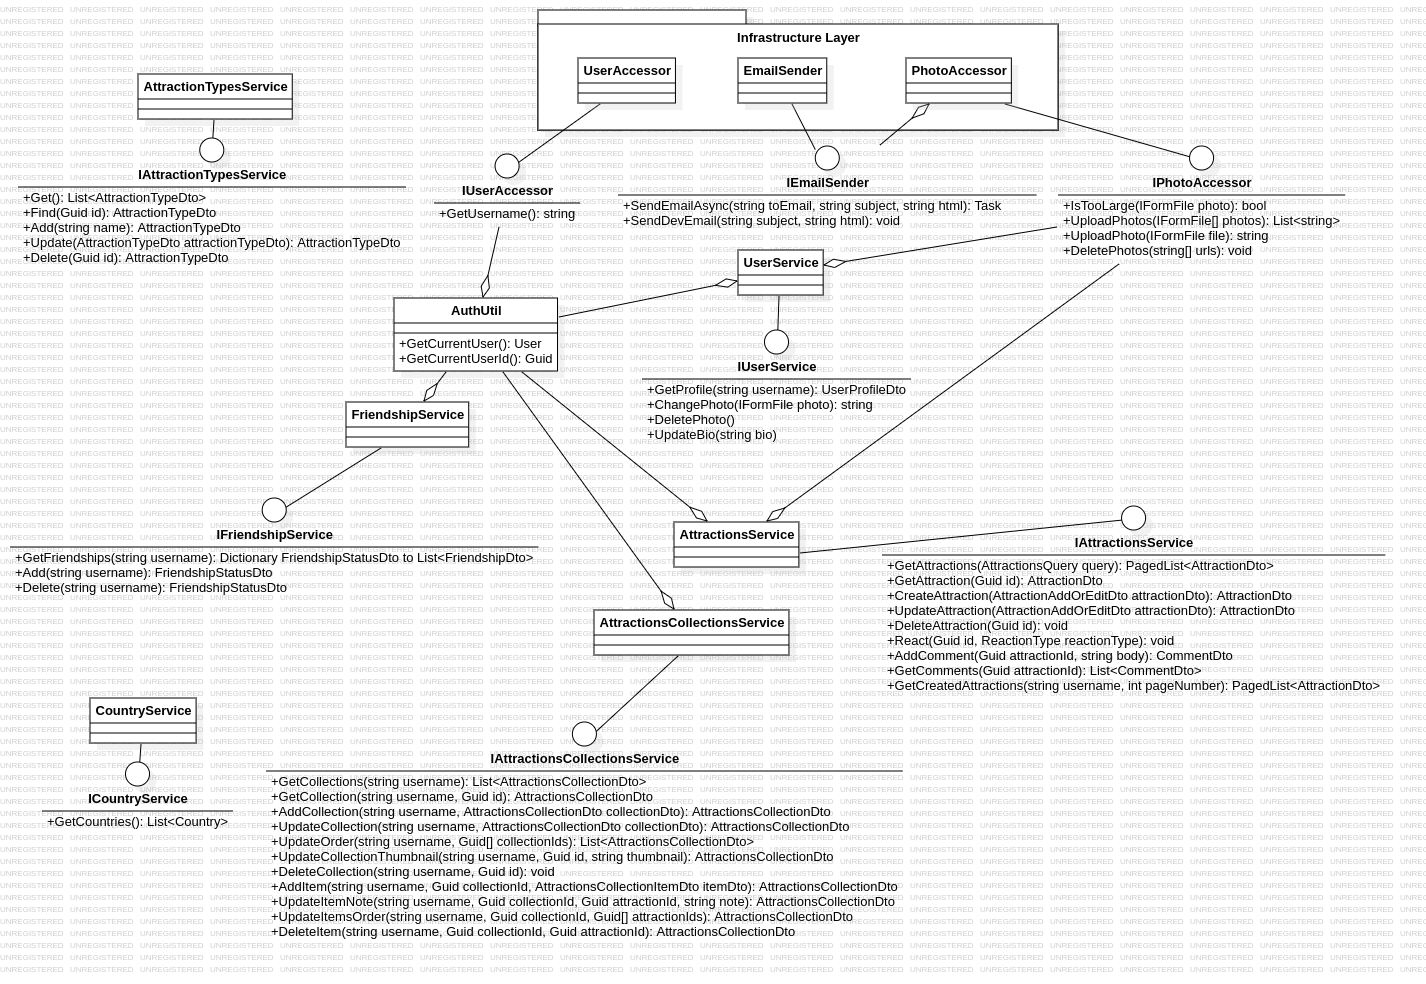
\includegraphics[width=1\linewidth]{business-class-diagram.png}
    \caption{Business logic class diagram}
    \label{fig:enter-label}
\end{figure}

\section{Implementation}

\subsection{ORM Mapping}

\par Entity Framework was used to map the domain classes to the database tables. In order to achieve that, the domain classes have to be used as type parameters for fields of type \textit{DbSet} inside a class that inherits from the framework's class \textit{DbContext}. In this case the class is \textit{IdentityDbContext} because it offers user management features and it is also a descendant of the \textit{DbContext} class. This \textit{IdentityDbContext} class takes as type parameters a class used for mapping the user, a class used for mapping the user role and the type of the primary key used for those two.

\begin{figure}[!ht]
    \centering
    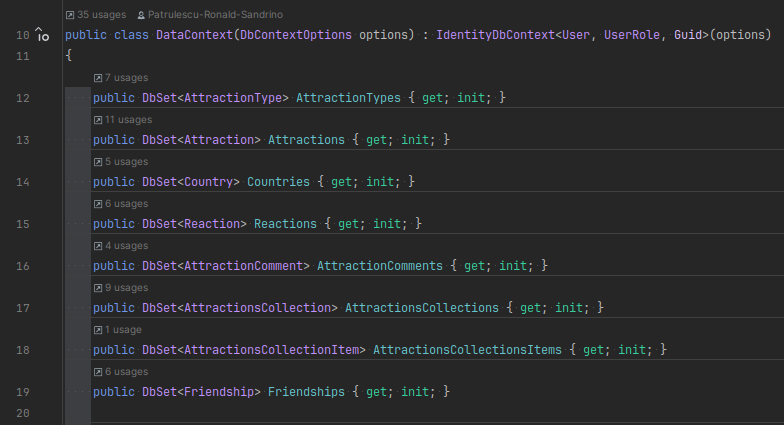
\includegraphics[width=1\linewidth]{4.3.1_dataContext.png}
    \caption{\textit{DataContext} class' fields}
    \label{fig:enter-label}
\end{figure}

\par The to be generated tables can be further configured by overriding the \textit{OnModelCreating} method of the \textit{DataContext} class. There you can define more complex primary keys, foreign keys, delete behaviors, unique indexes, check constraints, conversions, etc.

\clearpage % https://www.overleaf.com/learn/latex/Questions/How_can_I_get_my_table_or_figure_to_stay_where_they_are%2C_instead_of_going_to_the_next_page%3F

\begin{figure}[!ht]
    \centering
    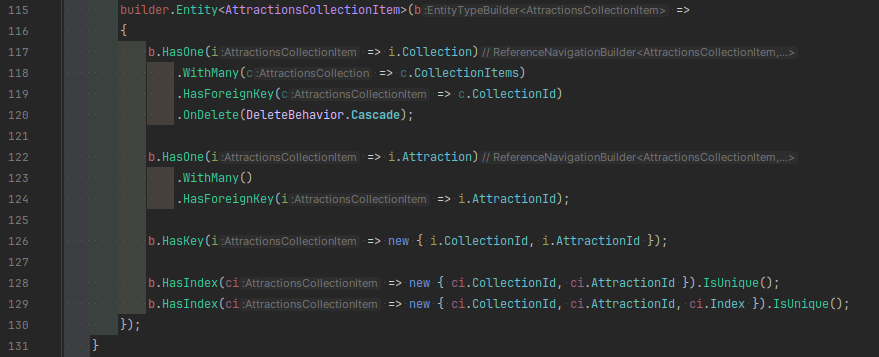
\includegraphics[width=0.95\linewidth]{4.3.1_sample-of-OnModelCreating.png}
    \caption{Example of configuring the database tables generation by overriding the \textit{OnModelCreating} method}
    \label{fig:enter-label}
\end{figure}

\par Furthermore, the defined \textit{DataContext} class has to be registered to the application services by using the \textit{AddDbContext} method. This also registers it for dependency injection so it can be used inside the service classes. This is also where the database provider is set up, which requires a method for registering it (which is usually provided by the package used for the database provider), \textit{UseSqlite} in this case, and a connection string.

\begin{figure}[!ht]
    \centering
    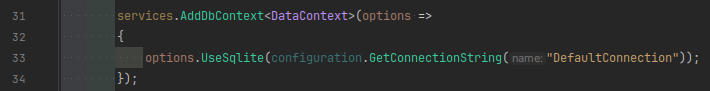
\includegraphics[width=1\linewidth]{4.3.1_AddDbContext.png}
    \caption{Registering the \textbf{DataContext} class}
    \label{fig:enter-label}
\end{figure}


\subsection{Automapper}

\par Automapper is an object-object mapper. It is used in this app in order to do conversions between domain classes and DTO classes. Mappings can be configured using profiles, which are classes that inherit from Automapper's Profile class. The profile is then registered to the DI container of application services:

\begin{figure}[!ht]
    \centering
    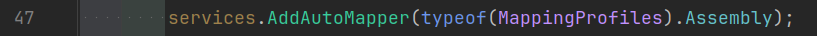
\includegraphics[width=1\linewidth]{4.3.2_automapper-injection.png}
    \caption{Registering Automapper to the application's DI container}
    \label{fig:automapper-injection}
\end{figure}

\clearpage % https://www.overleaf.com/learn/latex/Questions/How_can_I_get_my_table_or_figure_to_stay_where_they_are%2C_instead_of_going_to_the_next_page%3F

\par Mapping for fields with the same name happens implicitly. For the rest of them, we can define custom mappings or even ignore them, as seen in Figure \ref{fig:automapper-profile}, at lines 15 and 21 respectively.

\begin{figure}[!ht]
        \centering
        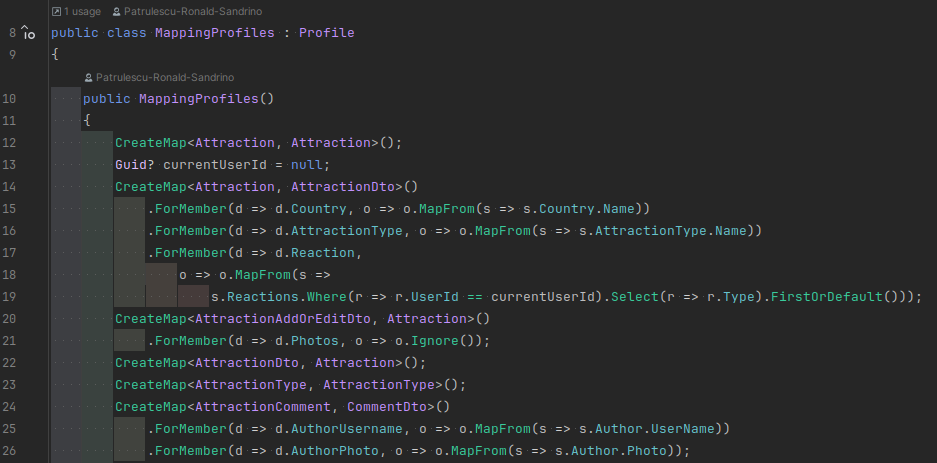
\includegraphics[width=1\linewidth]{4.3.2_automapper-profile.png}
        \caption{Example of Automapper profile configuration}
        \label{fig:automapper-profile}
\end{figure}

\begin{figure}[!ht]
    \centering
    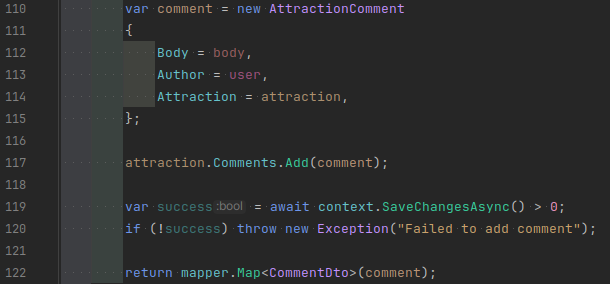
\includegraphics[width=1\linewidth]{4.3.2_automapper-usage.png}
    \caption{Example of Automapper usage (line 122)}
    \label{fig:automapper-usage}
\end{figure}


\subsection{Reading from and writing to the database}

\par Reading is done by directly accessing the \textit{DbSet} fields of the \textit{DataContext} class. For example, in Figure \ref{fig:database-read} at line 58 the contents of table of attraction types are accessed by the AttractionTypes field on the variable context, which is an instance of \textit{DataContext} injected into the service. The contents can be further processed on the database side by using non-terminal operations, methods that return an instance of \textit{IQueryable}, like Where, Include (which does join) and \textit{ProjectTo}. Then, when awaiting the call to \textit{ToListAsync} the processed query is performed on the database.

\begin{figure}[!ht]
    \centering
    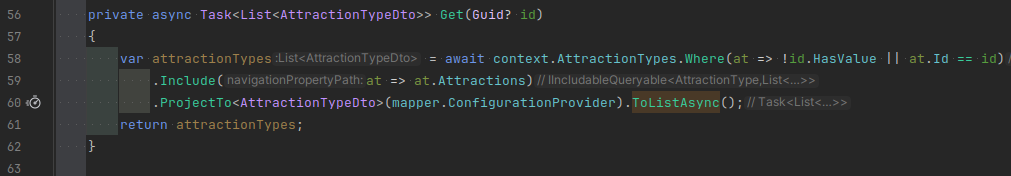
\includegraphics[width=1\linewidth]{4.3.3_database-read.png}
    \caption{Reading from the database}
    \label{fig:database-read}
\end{figure}

\par Writing to the database is done in 2 steps: 1. calling \textit{Add}/\textit{Remove} (and derivatives like \textit{AddAsync} or \textit{RemoveRange}) on either the \textit{DbSet} field or the DataContext instance, or by directly updating a domain class instance managed by the DataContext and which comes from a read operation and 2. by calling \textit{SaveChanges} on the \textit{DataContext} instances. An add example can be seen in Figure \ref{fig:automapper-usage} and an update example can be seen in Figure \ref{fig:database-write-update}

\begin{figure}[!ht]
    \centering
    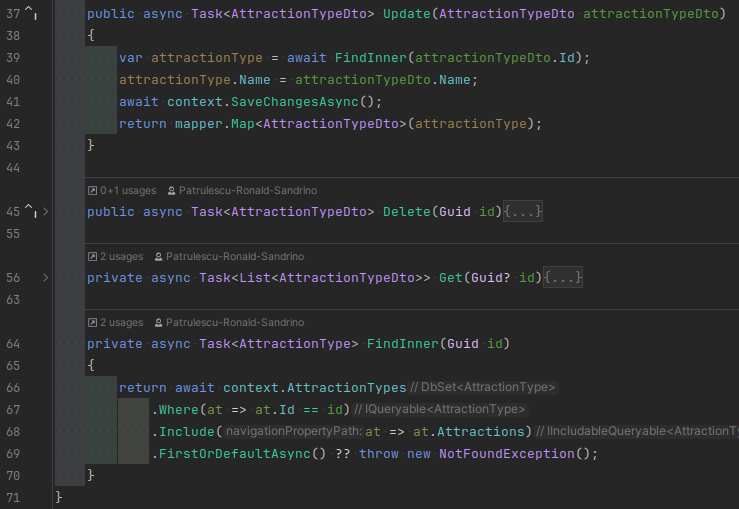
\includegraphics[width=1\linewidth]{4.3.3_database-write-update.png}
    \caption{Example of database update operation}
    \label{fig:database-write-update}
\end{figure}

\subsection{URL Mapping}

\par Each URL path is prefixed by the name of the controller. This is achieved by having all the controllers inherit from BaseApiController, which defines the path prefix using the Route annotation (Figure \ref{fig:url-mapping-baseapicontroller}). The rest of the URL path is defined by the argument of the annotations used for declaring the HTTP methods used (Figure \ref{fig:url-mapping-endpoints}). It can be observed that the paths can be parameterized.

\begin{figure}[!ht]
    \centering
    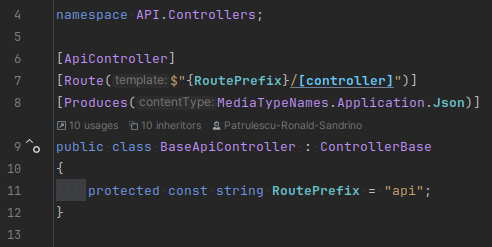
\includegraphics[width=1\linewidth]{4.3.4_url-mapping-baseapicontroller.png}
    \caption{How the name of the controller is added to the URL}
    \label{fig:url-mapping-baseapicontroller}
\end{figure}

\begin{figure}[!ht]
    \centering
    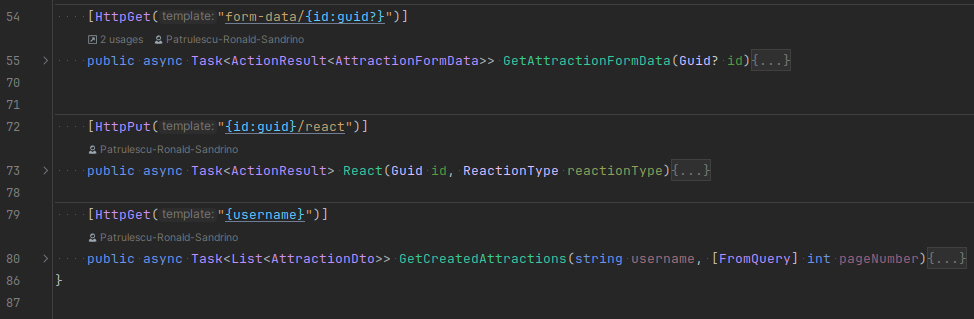
\includegraphics[width=1\linewidth]{4.3.4_url-mapping-endpoints.png}
    \caption{Defining endpoints}
    \label{fig:url-mapping-endpoints}
\end{figure}

\subsection{Dependency Injection}

\par Dependency injection is achieved by specifying the needed classes as constructor parameters (\ref{fig:dependency-injection_usage}) and then registering those classes when the application is created (\ref{fig:dependency-injection_registering}). Here, they are registered using the \textit{AddScoped} method, which registers their lifetime per HTTP request.


\begin{figure}[!ht]
    \centering
    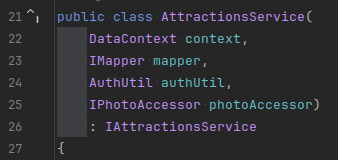
\includegraphics[width=0.5\linewidth]{dependency-injection_usage.png}
    \caption{Injection of dependencies using the primary constructor}
    \label{fig:dependency-injection_usage}
\end{figure}

\begin{figure}
    \centering
    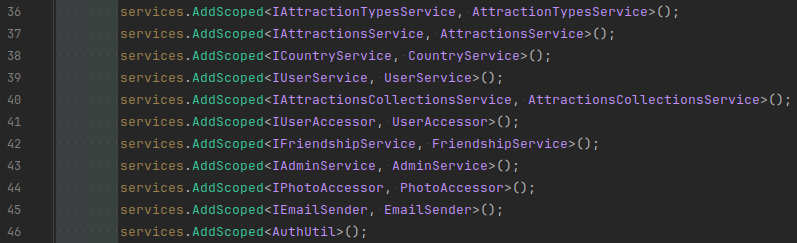
\includegraphics[width=1\linewidth]{dependency-injection_registering.png}
    \caption{Registration of dependencies}
    \label{fig:dependency-injection_registering}
\end{figure}

\subsection{Error handling}

\par When the Web API is created (in the entry point of the application - the \textit{Program.cs} file) there are 2 things that are done. The first one is the registration of the services (Figure \ref{fig:exception-handling_registration} lines 18 - 28) and the second is the configuration of the HTTP request pipeline (Figure \ref{fig:exception-handling_registration} lines 33 - ...). The order in which the middlewares are configured is the order in which they are run. And, the reason the exception handling middleware is the  first in the pipeline (Figure \ref{fig:exception-handling_registration} line 33) is to catch any exception that occurs later in the pipeline. The purpose of the exception middleware is to have a single piece of code that handles what response is given, depending on the exception, to the initiator of the HTTP request. In this application, it changes the status code depending on the exception (Figure \ref{fig:exception-handling_middleware} lines 24 - 33), writes the validation errors to the body of the response (Figure \ref{fig:exception-handling_middleware}) line  33) and adds the stacktrace to the response only if the app is running in development mode.

\begin{figure}
    \centering
    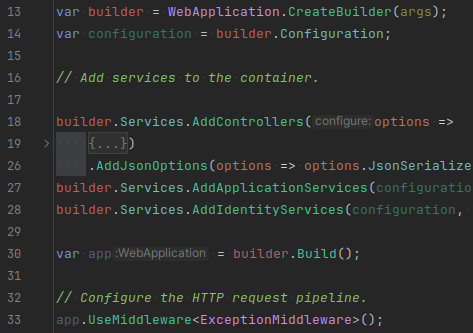
\includegraphics[width=1\linewidth]{exception-handling_registration.png}
    \caption{Registration of the exception handling middleware}
    \label{fig:exception-handling_registration}
\end{figure}

\begin{figure}
    \centering
    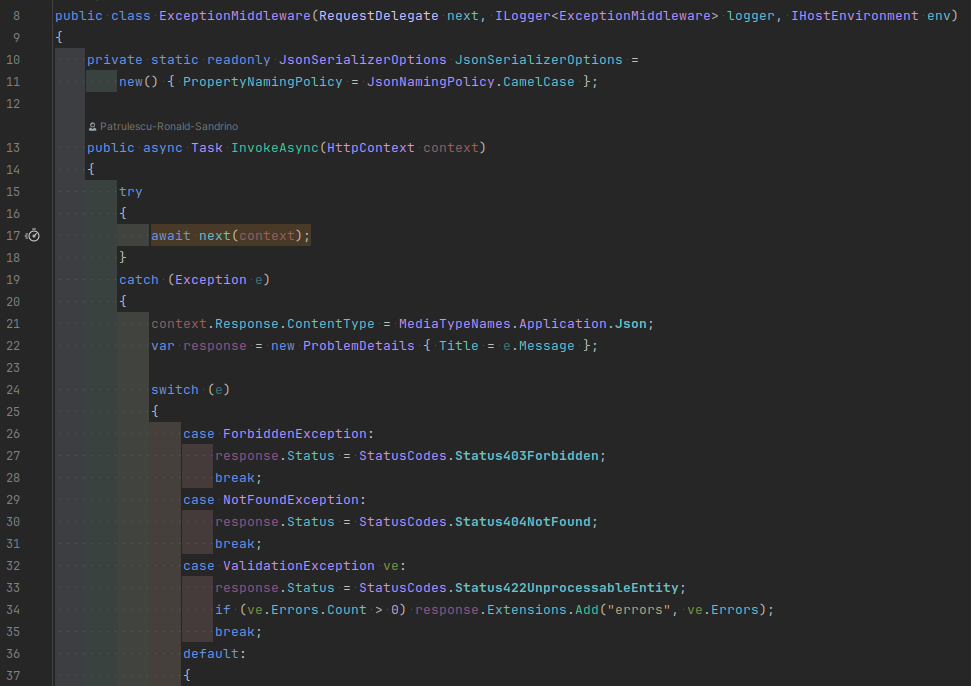
\includegraphics[width=1\linewidth]{exception-handling_middleware.png}
    \caption{Middleware for exception handling}
    \label{fig:exception-handling_middleware}
\end{figure}